\documentclass[../../main.tex]{subfiles}

\begin{document}

\section{Variabili cinematiche}
La \textbf{traiettoria} di un punto P in moto, è in generale una \textit{linea curva}.
\subsection{Posizione}
Dato un sistema di riferimento cartesiano con origine in O e assi x, y, z, la posizione di un punto P è definita da un vettore $\bar{r}$ che congiunge l'origine con un punto P. Dato che il punto P si muove, la posizione è una funzione del tempo:
\[ \bar{r} = \bar{r}(t) \]
$r$ può essere espresso in forma cartesiana attraverso le sue componenti $x, y, z$:
\[ \bar{r}(t) = \textbf{OP} = x(t)\bar{u}_x + y(t)\bar{u}_y + z(t)\bar{u}_z \]
Conoscere $r(t)$ signifca conoscere $x(t)$, $y(t)$ e $z(t)$: le leggi orarie.

\begin{figure}[h!]
    \centering
    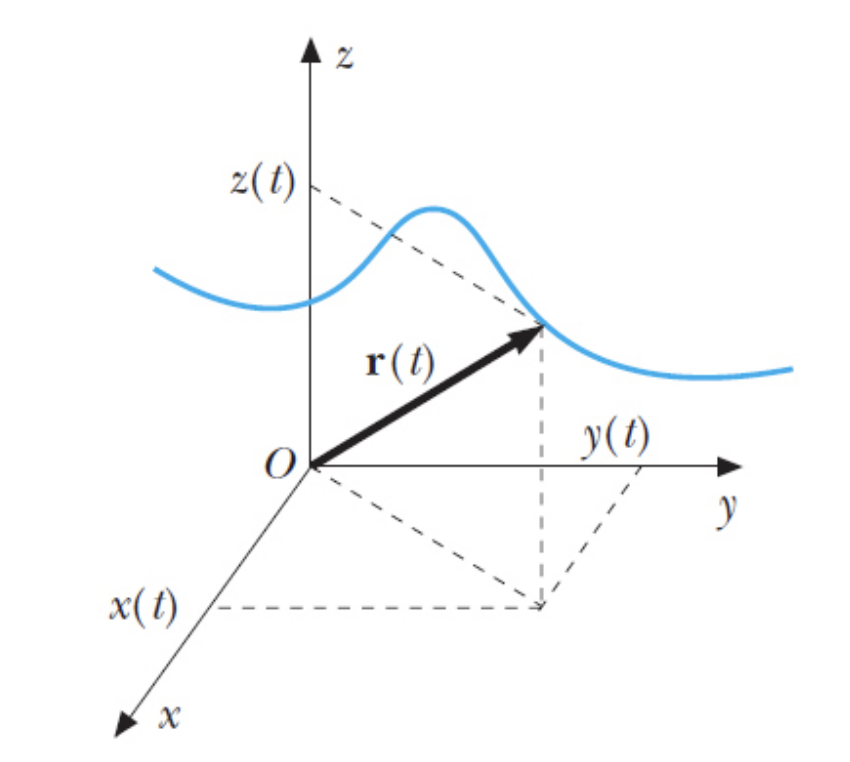
\includegraphics[width=0.5\textwidth]{traiettoria.png}
    \caption{Traiettoria di un punto}
\end{figure}
$\bar{r}(t)$ o $\overline{OP}$ vettore posizione o raggio vettore.
\[
    \bar r(t) = x(t)\bar{u}_x + y(t)\bar{u}_y + z(t)\bar{u}_z \ \ \ \textit{Legge oraria}
\]

\subsection{Velocità}
Consideriamo due posizioni occupate dal punto P in due istanti di tempo diversi $t$ e $t + \Delta t$: esse sono individuate dai vettori $\textbf{r}(t)$ e $\textbf{r}(t + \Delta t) = \textbf{r}(t) + \Delta \textbf{r}$. Il vettore:
\[ \Delta \textbf{r} = \textbf{r}(t + \Delta t) - \textbf{r}(t) \]
è il \textbf{vettore spostamento} del punto P nell'intervallo di tempo $\Delta t$.\\
La velocità media è definita come:
\[ \bar{v}_m = \dfrac{\Delta \bar{r}}{\Delta t} \]
\begin{figure}[h!]
    \centering
    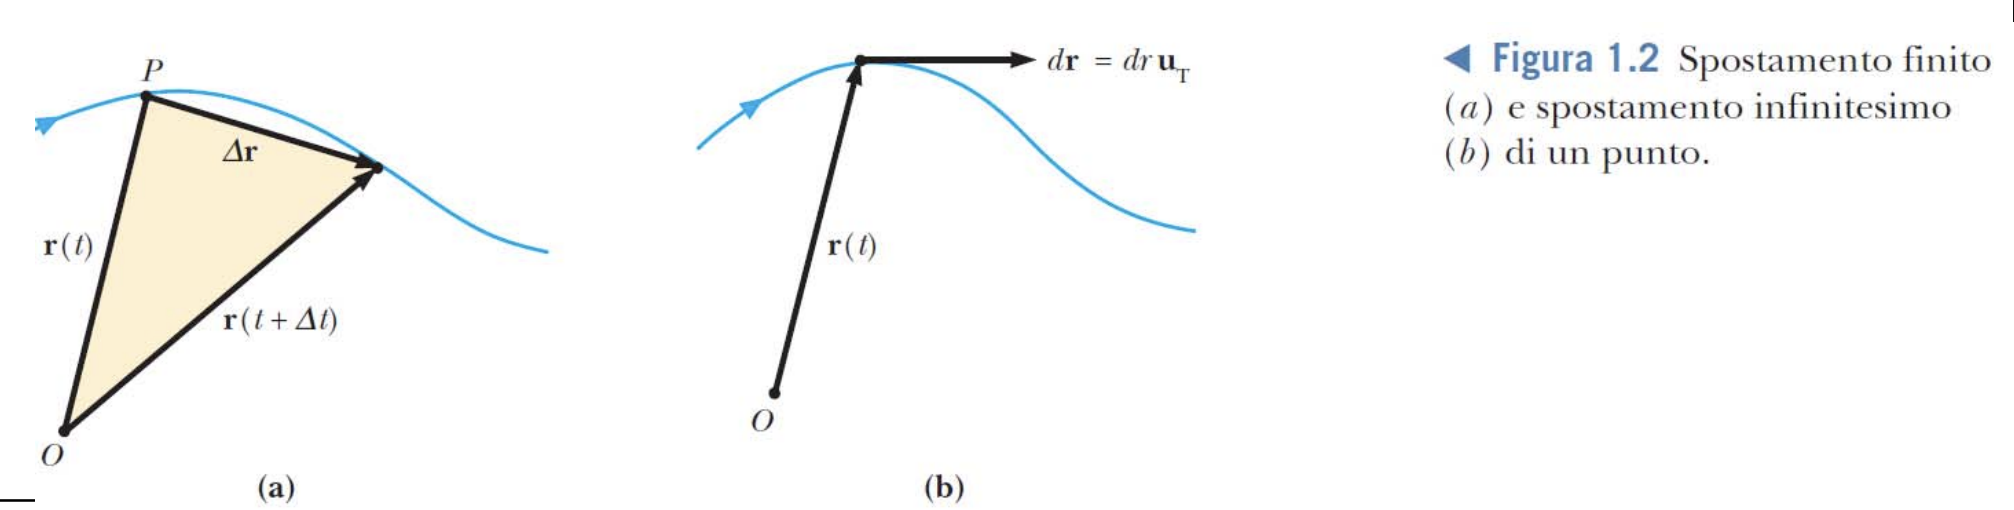
\includegraphics[width=0.5\textwidth]{velocitatangente.png}
    \label{fig:velocitatangente}
\end{figure}
La velocità media è un vettore parallelo allo spostamento, ed esprime la rapidità con cui il punto P si sposta da un punto all'altro.
Essa dà informazioni complessive senza fornire nessuna indicazione di come avviene il moto nell'intervallo di tempo $\Delta t$.\\
Per ovviare a questa indeterminazione si può ridurre l'intervallo di tempo $\Delta t$ fino a renderlo infinitesimo, ottenendo la \textbf{velocità istantanea}:
\[ \bar{v} = \lim_{\Delta t \to 0} \dfrac{\Delta \bar{r}}{\Delta t} = \dfrac{d\bar{r}}{dt} \]
La velocità è anch'essa un vettore e rappresenta la rapidità di variazione temporale della posizione nell'istante $t$.

Osserviamo che (figura \ref{fig:velocitatangente}) al limite l'incremento $d\bar{r}$ infinitesimo del raggio vettore risulta in \textit{direzione tangente alla traiettoria nel punto} P.\\
La velocità è sempre tangente alla traiettoria:
\[
    \bar{v}_m = \dfrac{\bar{r}(t + \Delta t) - \bar{r}(t)}{\Delta t} \ \ \ \textit{Velocità media}
\]
\[
    \bar{v} = \lim_{\Delta t \to 0} \dfrac{\bar{r}(t + \Delta t) - \bar{r}(t)}{\Delta t} = \dfrac{d\bar{r}}{dt} \ \ \ \textit{Derivata del vettore posizione}
\]
\subsection{Componenti cartesiane della velocità}
Poichè $\bar r = x\bar{u}_x + y\bar{u}_y + z\bar{u}_z$:
\[
    \bar{v} = \dfrac{dx}{dt} \bar{u}_x + \dfrac{dy}{dt} \bar{u}_y + \dfrac{dz}{dt} \bar{u}_z = v_x\bar{u}_x + v_y\bar{u}_y + v_z\bar{u}_z
\]
La velocità è determinata se sono note le derivare delle tre coordinate $x(t)$, $y(t)$, $z(t)$.
\begin{figure}[H]
    \centering
    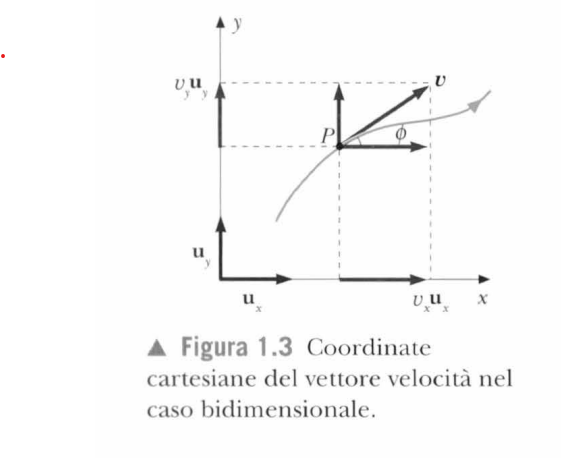
\includegraphics[width=0.5\textwidth]{coordinate_cartesiane.png}
\end{figure}
Per esempio posso ottenere $v_x = v\cos\phi_x$. Nel caso bidimensionale è necessario un solo angolo.
Lo spostamento può essere trovato come differenza tra il vettore di posizione finale e quello iniziale:
\begin{figure}[H]
    \centering
    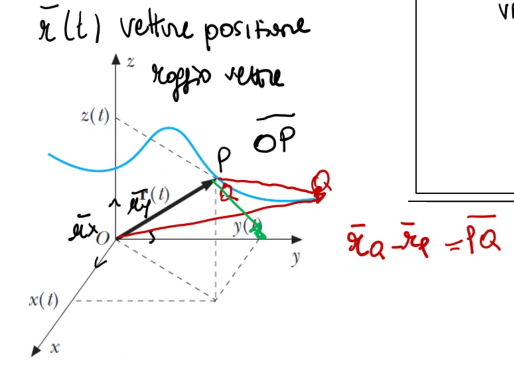
\includegraphics[width=0.5\textwidth]{posizionevettore.png}
\end{figure}
\[
    \overline{r_q} - \overline{r_p} = \overline{PQ}
\]
Se conosco la velocità posso ricavare il vettore posizione:
\[
    dr = \bar{v}dt \implies \int_{\bar{r}_0}^{\bar{r}} dr = \int_{t_0}^{t} \bar{v}dt = \bar{r} - \bar{r}_0 = \int_{t_0}^{t} \bar{v}dt \implies
\]
\[
    \bar{r} = \bar{r}_0 + \int_{t_0}^{t} \bar{v_x}dt\bar{u}_x \ldots
\]
\subsection{Accelerazione}


\subsection{Componenti cartesiane dell'accelerazione}


\subsection{Coordinate polari}
Nel moto su di un piano la posizione del punto viene individuata da due coordinate. Esse possono essere, con riferimento ad un sistema di assi cartesiani, le coordinate cartesiane $x(t)$, $y(t)$ oppure le coordinate polari $r(t)$, $\theta(t)$. Le relazioni che intercorrono tra le coordinate cartesiane e quelle polari sono:
\[
    \begin{cases}
        x = r\cos\theta \\
        y = r\sin\theta
    \end{cases}
    \iff r = \sqrt{x^2 + y^2} \ \ \ \tan\theta = \dfrac{y}{x}
\]
\begin{minipage}{0.5\textwidth}
    \centering
    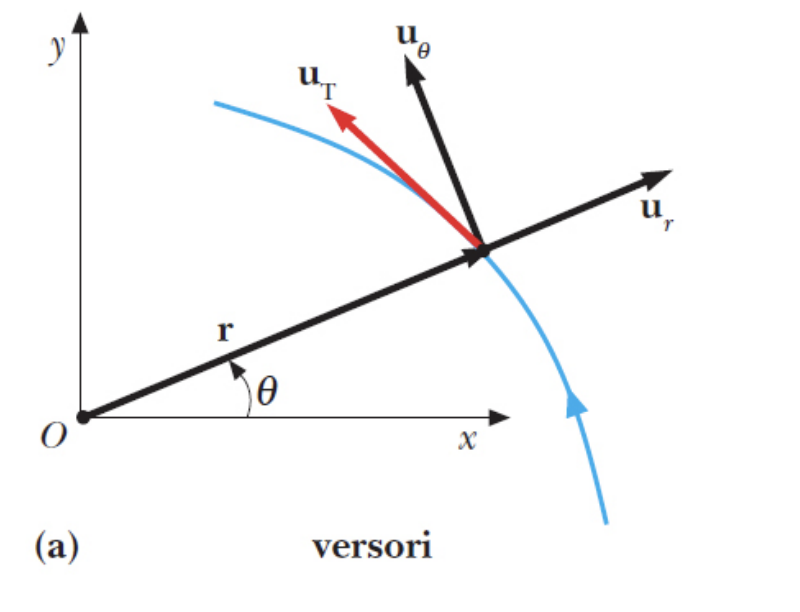
\includegraphics[width=0.5\textwidth]{polare1.png}
\end{minipage}
\begin{minipage}{0.5\textwidth}
    \centering
    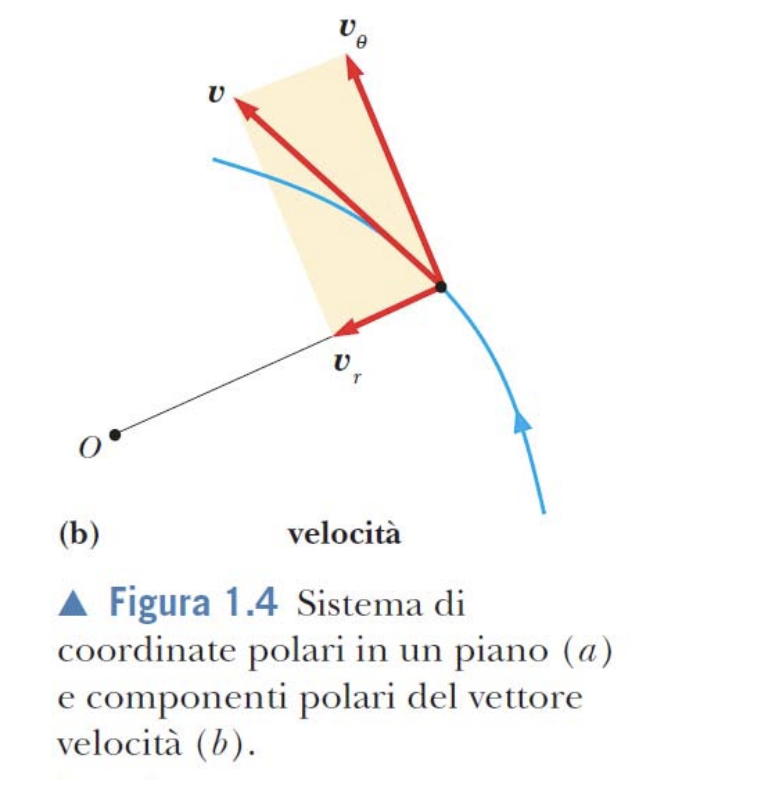
\includegraphics[width=0.5\textwidth]{polare2.png}
\end{minipage}

\subsection{Componenti polari della velocità}
I vettori $\bar{u}_r$ e $\bar{u}_\theta$, sono versori della direzione di $\bar r$ e versore ortogonale alla stessa: si noti che questi versori cambiano verso durante il moto.\\
Il raggio vettore $\bar r$ può essere espresso come $r\bar r_r$ e pertanto:
\[
    \bar v = \dfrac{d\bar r}{dt} = \dfrac{dr}{dt}\bar u_r + r\dfrac{d\bar u_r}{dt} \implies \bar v = \dfrac{dr}{dt}\bar u_r + r\dfrac{d\theta}{dt}\bar u_\theta = \bar v_r + \bar v_\theta
\]
\[
    u_\theta = \textit{ versore trasverso}
\]
\[
    u_r = \textit{ versore radiale}
\]









\end{document}